\documentclass[12pt, A4]{report}

% Packages
	% Basics
		\usepackage{amsmath}
		\usepackage{bm}
		\usepackage{cellspace}
		\usepackage{csquotes}
		\usepackage{fixltx2e}
		\usepackage[hang,flushmargin]{footmisc}
		\usepackage{float}
		\usepackage[margin=0.75in]{geometry}
		\usepackage{graphicx}
		\usepackage{hyperref}
		\usepackage[utf8]{inputenc}
		\usepackage{subcaption}
	% Diagrams
		\usepackage{pgfplots}
		\usepackage{tikz}
			\usepackage{circuitikz} % Circuits
			\usepackage{tikz-3dplot} % 3D
			\usetikzlibrary{arrows.meta, angles, calc, quotes}
	% Notation
		\usepackage{amssymb} % Miscellaneous
		\usepackage{chemformula}
		\usepackage{esint} % Integrals
		\usepackage{physics} % Differentials/Vectors
% Configuration
	\title{Use of Stochastic Calculus to Predict Stock Market Trends}
	\author{Arnav Patri and Shashank Chidige}
	\date{}
	\hypersetup{
	    colorlinks,
	    citecolor=cyan,
	    filecolor=cyan,
	    linkcolor=cyan,
	    urlcolor=cyan
	}
	\cellspacetoplimit10pt
	\cellspacebottomlimit10pt
	
% Macros
	% Notation
		% Constants
			\DeclareMathOperator{\en}{e}
		% Distributions
			\newcommand{\Exp}{\mathbb{E}}
			\newcommand{\ndist}{\mathcal{N}}
			\DeclareMathOperator{\vari}{var}
		% Functions
			\DeclareMathOperator{\erfc}{erfc}
		% Sets
			\newcommand{\R}{\mathbb{R}}
		% Other
			\DeclareMathOperator{\avg}{avg}
			\renewcommand{\th}{\text{th}}
	% Utilities
		\newcommand{\callout}[2]{\begin{center}\fbox{\begin{minipage}{#1cm}#2\end{minipage}}\end{center}}
		\newcommand{\comment}[1]{}
		\newcommand{\subsectionb}[1]{\subsection*{#1}\addcontentsline{toc}{subsection}{#1}}
		\newcommand{\subsubsectionb}[1]{\subsubsection*{#1}\addcontentsline{toc}{subsubsection}{#1}}
		
\begin{document}
	\maketitle
	\noindent
		\maketitle
	\noindent
	The aim of this project is to use differential equations to determine a method by which the behavior of stock prices can be modeled to gain financial insight. There are simply too many variables that have an impact on a stock's price, though, not all of which can be individually accounted for. The problem of optimizing buy and sell times of stocks is affected by the multitude of internal and external forces that affect the stock's price. In business, political, economic, social, and technological changes in the business environment can impact a stock's price. Rather than attempting to account for every individual variable, the aggregate result can be modeled stochastically. \\
	Despite its complexity, an understanding of both statistics and differential equations being required, stochastic calculus enables traders to make more informed predictions regarding stock prices. Many firms already employ stochastic models for this reason. They stand to gain financially by increasing the accuracy of their prediction. In fact, many trading services directly incorporate stochastic models unbeknownst to those using them. \\
	The model being employed is
		\[\dv{S_t}{t} = \mu S_t + \sigma S_t\dv{W_t}{t}\]
		where \(t\) is time (the independent variable), \(S_t\) is the stock price (as a function of time), \(\mu\) is the (constant) expected return on the stock, \(\sigma\) is the (constant) volatility (standard deviation), and \(W_t\) is a standard Wiener process, with mean 0 and variance 1, as adapted from \cite{Stochastic}: \\
		The Wiener process is stochastic, meaning that its value changes over time randomly. As such, only the distribution of possible values is known at any given point in time. This distribution is defined by the mean and variance, in this case 0 and 1 respectively. The Wiener process is a series of randomly distributed normal variables with variances that increase over time, reflecting the increasing uncertainty in making predictions further into the future. \\
		The change in the Wiener process can be found as
		\[\Delta W = \varepsilon\sqrt{\Delta t}\]
		where \(\varepsilon \sim \ndist(0, 1)\) (\(\varepsilon\) being a continuous random variable following the standard Normal distribution, but mean 0 and variance 1). This implies that the change in the Wiener process is itself a transformation of the standard Normal distribution, as \(\sqrt{\Delta t}\) is simply some constant multiplier when parameter \(t\) is fixed. \\
		As such, the mean of the Wiener process (its expected value \(\Exp[W_t]\)) can be found to be
			\[\Exp[\Delta W] = \sqrt{\Delta t} \times \Exp[\varepsilon] = 0\]
		and its variance
			\[\vari[x] = \left(\sqrt{\Delta t}\right)^2\vari[\varepsilon] = \Delta t\]
		The Wiener process can therefore be denoted \(\ndist(0, \Delta t)\). \\
		The difference between the Wiener process at times \(T\) and 0 can be found as
		\[W(T) - W(0) = \sum_{i = 1}^n \varepsilon_i\sqrt{\Delta t} = \sum_{i = 1}^n W_i \quad \text{where } n = \frac{T}{\Delta t} \]
		As \(W(T) - W(0)\) is simply a linear combination of \(n\) random normal variables \(W_i\), it must itself also follow a Normal distribution. It should be noted that \(W(0)\) must be fixed, as it is what defines the function's starting point. As such,
		\[\Exp[W(0)] = \vari[W(0)] = 0\]
 		It can then be seen that
 		\[\Exp[W(T) - W(0)] = \Exp[W(T)] - \Exp[W(0)] = \Exp[W(T)]\]
 		As the difference is a linear combination of \(\Delta W_t\) \(n\) times,
 			\[\Exp[W(T)] = n \times \Exp[\Delta W_t] = 0\]
 		The distributions of the values Wiener process at times \(t_i\) and \(t_j\) are independent, so
 			\[\vari[W(T) - W(0)] = \vari[W(T)] + \vari[W(0)] = \vari[W(T)] = n \times \vari[\Delta W_t] = n\Delta t\]
 		In conclusion, \(W(T) \sim \ndist(0, T)\). \\
		 As \(n \to \infty\), \(\Delta t\) and \(\Delta W_t\) become the differentials \(\dd{t}\) and \(\dd{W_t}\).
	The only conditions that the model must follow are that the stock price and time cannot fall below 0. Note the lack of an upper bound to the stock's price.
	\par\noindent\rule{\textwidth}{0.5mm}
	Table 1 shows information regarding Alphabet Inc., which is listed on the New York Stock Exchange as GOOG, as the company used to be known as Google. The data is taken from Yahoo Finance \cite{Yahoo}, which provides financial news and data for public use. The domain of the independent variable, time (\(t\)) is taken from 9/27/2022 to 10/15/2022.
	\[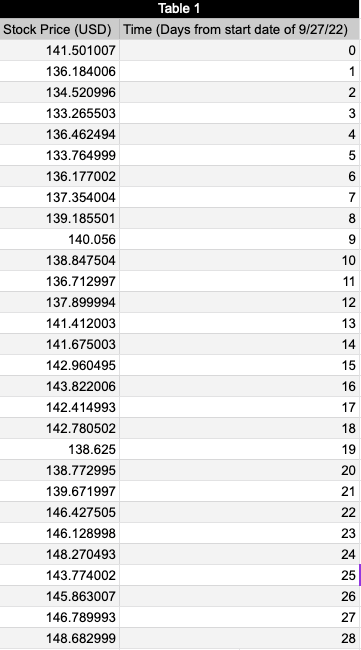
\includegraphics[width = 8cm]{Images/Table_1}\]
	Table 2 shows the differential approach to deriving the differential equation model. As the stochastic part cannot be derived, only the derivation of the deterministic part is shown. Columns 1 and 2 are simply copied from Table 1. Equations 1 and 2 are used to derive the changes in stock price \(S_t\) and time \(t\), put into columns 3 and 4 respectively. The derivative of \(S_t\) with respect to \(t\) can be approximated as \(\Delta S_t/\Delta t\), as shown in column 5. The stock price \(S_t\) is then listed again, as the plot is of \(\Delta S_t/\Delta t\) vs \(S_t\).
	\[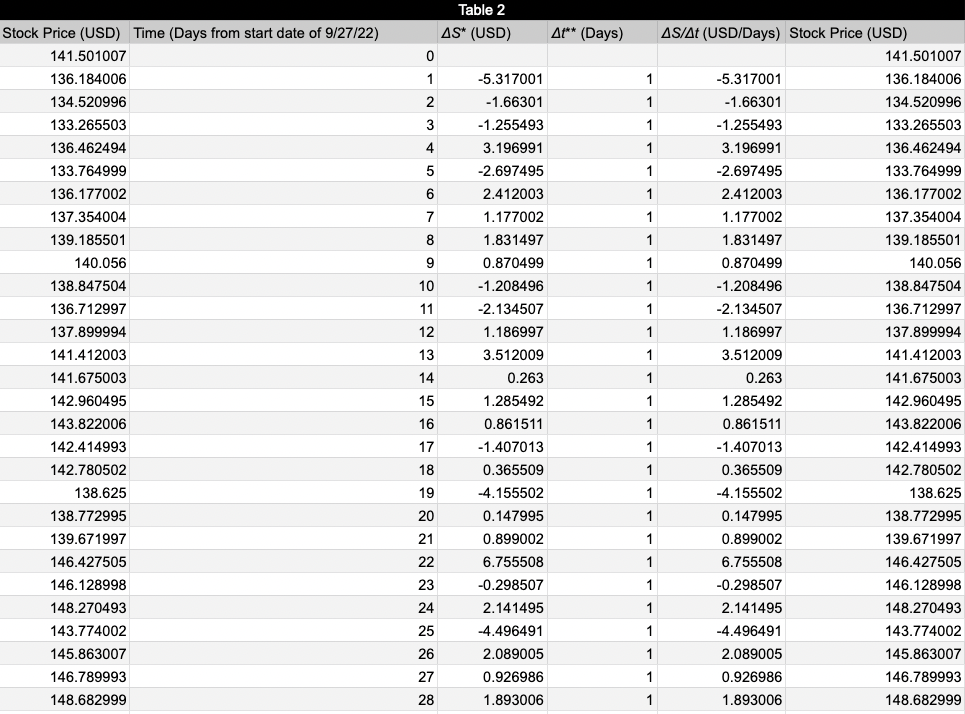
\includegraphics[width = 18cm]{Images/Table_2}\]
	\begin{align*}
		\Delta S_{t, i} &= S_{t, i} - S_{t, i - 1} \tag{Equation \(1^{*}\)} \\
		\Delta t_i &= t_i - t_{i - 1} \tag{Equation \(2^{**}\)}
	\end{align*}
	This is the graph of \(\Delta S/\Delta t\) (in USD/day) vs \(S\) (in USD), using data from Table 2, with a linear regression performed.
	\[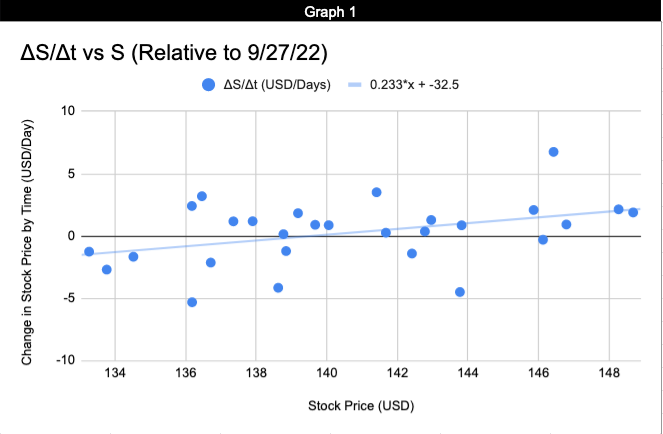
\includegraphics[width = 10cm]{Images/Graph_1}\]
	It is clear that there is a linear relationships between the stock price and its derivative with respect to time. It can therefore be said that
		\[\dv{S_t}{t} \propto S_t \implies \dv{S_t}{t} = \mu S_t\]
		where \(\mu\) is a constant. Using information from \cite{Stochastic}, the Wiener process can be appended, adding the random motion to the model:
		\[\dv{S_t}{t} = \mu S_t + \sigma S_t\dv{W_t}{t}\]
		where \(S_t\) is stock price as a function of time \(t\), \(\mu\) is the (constant) drift, \(\sigma\) is the (constant) volatility, and \(W_t\) is a standard Wiener process. \\
		The Wiener process is stochastic, meaning that its value changes over time randomly. As such, only the distribution of possible values is known at any given point in time. This distribution is defined by the mean and variance, in this case 0 and 1 respectively. The Wiener process is a series of randomly distributed normal variables with variances that increase over time, reflecting the increasing uncertainty in making predictions further into the future. \\
		The dependent variable \(t\) is not present, making this an autonomous DE. The only information needed for the model are \(\mu\), \(\sigma\), and the initial stock price \(S_0\). \\
	\(\mu\) is the amount that \(\Exp(S_t)\), the expected value of the stock price, changes per year, making it the coefficient of the linear regression of \(\Delta S_t/\Delta t\) against \(S_t\) divided by 365, so \(\mu \approx 0.00064\).\\
	\(\sigma\) is simply the standard deviation of the stock price in the sample, so 
		\[\sigma = \sqrt{\frac{\sum\limits_{i = 1}^n(S_{t, i} - \bar{S}_{t})^2}{n - 1}} \approx 4.356\]
		where \(n\) is the number of days sampled, \(S_{t, 1 \cdots n}\) are the particular stock prices, and \(\bar{S}_t\) is the average stock price in the sample:
		\[\bar{S}_t = \frac{\sum\limits_{i = 1}^nS_{t,i}}{n}\]
	The model then becomes
		\[\boxed{\dv{S_t}{t} = 0.00064S_t + 4.356S_t\dv{W_t}{t}}\]
		\par\noindent\rule{\textwidth}{0.5mm}
		\comment{
			The following is the \href{https://docs.google.com/spreadsheets/d/10UhPew6GsC5f6DCJjFd24MZSaZ1SWjiQvmOD6k-tmcE/edit}{\underline{Excel spreadsheet}}. It uses data collected from Yahoo Finance on the value of GOOG (Alphabet Inc.'s stock price). \\
			A stock's price \(S_t\) (in USD) can be predicted with respect to time \(t\) (in days from an initial time) using a growth function; that is, by relating the rate at which the stock price is changing to the current stock price as a proportion:
				\[\dv{S_t}{t} \propto S_t\]
				The constant of proportionality is the drift \(\mu\) of the stock, which is the rate of change of the expected value \(\Exp[S_t]\) of the stock price with respect to time (which is not the expected value of its rate of change):
				\[
					\dv{S_t}{t} = \mu S_t \qquad \text{where} \qquad
					\mu= \frac{\Delta \Exp[S_t]}{\Delta t}
				\]
				The stock market is constantly volatile, though, changing in unpredictable ways. This randomness element can be modeled by a randomness term, proportional to the product of the stock price and the rate of change of the standard Wiener process \(W_t\) (as defined in Phase 2):
				\[\text{rate of randomness} \propto S_t\dv{W_t}{t}\]
				The proportionality constant is the volatility \(\sigma\) of the stock, which is simply its standard deviation. Adding this term,
				\[
					\dv{S_t}{t} = \mu S_t + \sigma S_t\dv{W_t}{t} \qquad \text{where} \qquad
					\sigma = \frac{\sum (S_{t, i} - \bar{S_t})}{n - 1} \qquad \text{and} \qquad
					\bar{S_t} = \frac{\sum S_{t, i}}{n}
				\]
		}
		The randomness term ensures that each trial of the model yields a different graph. One such trial is attached at the end of this document.
		\subsubsection*{It\^o's Lemma and Separation of Variables}
		\noindent \\ The DE 
			\[\dv{S_t}{t} = \mu S_t + \sigma S_t\dv{W_t}{t}\]
			where \(S_t\) is stock price (the dependent variable in USD) as a function of time \(t\) (the independent variable in days), \(\mu\) is the (constant) drift, \(\sigma\) is the (constant) volatility, and \(W_t\) is a standard Wiener process (written in terms of the parameters solved for previously) can be rewritten as
			\[\dd{S}_t = \mu_t\dd{t} + \sigma_t\dd{W_t}\]
			where \(\mu_t = \mu S_t\) and \(\sigma_t = \sigma S_t\). Integrating and reparameterizing \(\mu_t\), \(\sigma_t\) and \(W_t\) with \(s\),
			\[S_t = \int_0^t\mu_s\dd{s} + \int_0^t\sigma_s\dd{W}_s + C\]
			where \(C\) is the constant of integration. This makes \(S_t\) an It\^o process, a stochastic process expressible as the sum of two integrals, one with respect to a stochastic process and another with respect to time, and a constant. \\
		The Taylor expansion of a twice-differentiable scalar function \(f(t, s)\) is
			\[\dd{f} = \pdv{f}{t}\dd{t} + \pdv{f}{s}\dd{s} + \frac{1}{2}\pdv[2]{f}{s}\dd[2]{s} + \cdots\]
			Substituting \(S_t\) for \(s\) and appropriately substituting for \(\dd{s}\) yields
			\[\dd{f} + \pdv{f}{t}\dd{t} + \pdv{f}{s} (\mu_t\dd{t} + \sigma_t\dd{W_t}) + \pdv[2]{f}{s}\left(\mu_t^2\dd{t^2} + 2\mu_t\sigma_t\dd{t}\dd{W_t} + \sigma_t^2\dd{W_t}^2\right) + \cdots\]
			As \(\dd{t}\) approaches 0, \(\dd{t}^2\) and \(\dd{t}\dd{W_t}\) tend to zero faster than \(\dd{W_t^2}\). Substituting 0 for \(\dd{t^2}\) and \(\dd{t}\dd{W_t}\) and \(\dd{t}\) for \(\dd{W_t^2}\) yields
			\[\dd{f} = \left(\pdv{f}{t} + \mu_t\pdv{f}{s} + \frac{\sigma_t^2}{2}\pdv[2]{f}{s}\right)\dd{t} + \sigma_t\pdv{f}{s}\dd{W_t}\]
			This is itself an It\^o process. It\^o's lemma states that for any It\^o process \(S_t\) and any twice-differentiable function \(f(t, s)\), \(f(t, S_t)\) is an It\^o process. \\
		Let \(f(S_t) = \ln S_t\). Applying It\^o's lemma,
			\begin{align*}
				\dd{f} &= f'(S_t)\dd{S_t} + \frac{1}{2}f''(S_t)(\dd{S_t})^2 \\
					&= \frac{1}{S_t}\dd{S_t} - \frac{1}{2S_2^2}\left(S_t^2\sigma^2\dd{t}\right) \\
					&= \frac{1}{S_t}(\sigma S_1 \dd{W_t} + \mu S_t \dd{t}) - \frac{\sigma^2}{2}\dd{t} \\
					&= \sigma \dd{W_t} + \left(\mu - \frac{\sigma^2}{2}\right)\dd{t}
			\end{align*}
			The Wiener process greatly limits the possibilities for solving this DE. It is inexact, nonlinear, and nonhomogenous. The integrating factor cannot be used either due to the Wiener process. As such, separation of variables is the only suitable method. Integrating the separable DE,
			\[
				f(t) = \ln S_t 
					= \ln C + \sigma W_t + \left(\mu - \frac{\sigma^2}{2}\right)\dd{t} \\
			\]
			This can finally be exponentiated, yielding \(S_t\):
			\[S_t = C\en^{\left(\mu - \frac{\sigma^2}{2}\right)t + \sigma W_t}\]
			(This method of solution was largely adapted from \cite{Ito} and \cite{Brownian}) \\
			Applying the initial condition \(S_t(0) = S_0\), the initial stock price of \$141.501. Letting \(t = 0\),
			\[S_t(0) = Ce^{\sigma W_t}\] 
			At time \(t = 0\), the randomness from the Wiener process does not have any affect, is it only takes hold as \(t\) gets further from the initial time of 0. As such, it is equal to 0, so
			\[
				S_t(0) = C
					= S_0
					= \$141.501
			\]
			Substituting for \(\mu\) and \(\sigma\),
			\[\boxed{S_t = 141.501\en^{\left(0.00064 + \frac{4.356^2}{2}\right)t + 4.356W_t} = 141.501\en^{9.488t + 4.356W_t}}\]
			It should be noted that the Stock's price may not fall below 0, as the solution is an exponential with a positive coefficient. \\
			Below is the graph of the solution in Excel:
				\[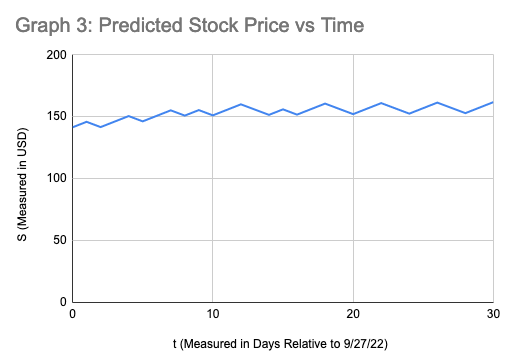
\includegraphics[width = 8cm]{images/Graph_2.png}\]
				the randomness term was simulated using the random walk approach (adapted from \cite{Random}), generating random numbers and compounding the change between them to create a random process with uncertainty that increases with time.
			The following are the MatLab code, solution (for the deterministic term), and graph of the model of \(S_t\) vs \(t\):
				\[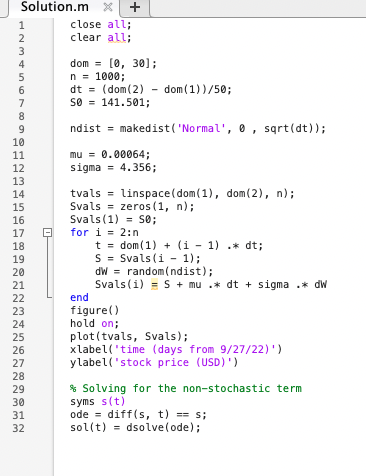
\includegraphics[width = 8cm]{Images/matlab.png}\]
				\[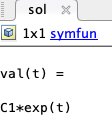
\includegraphics[width = 2cm]{Images/sol.png}\]
				\[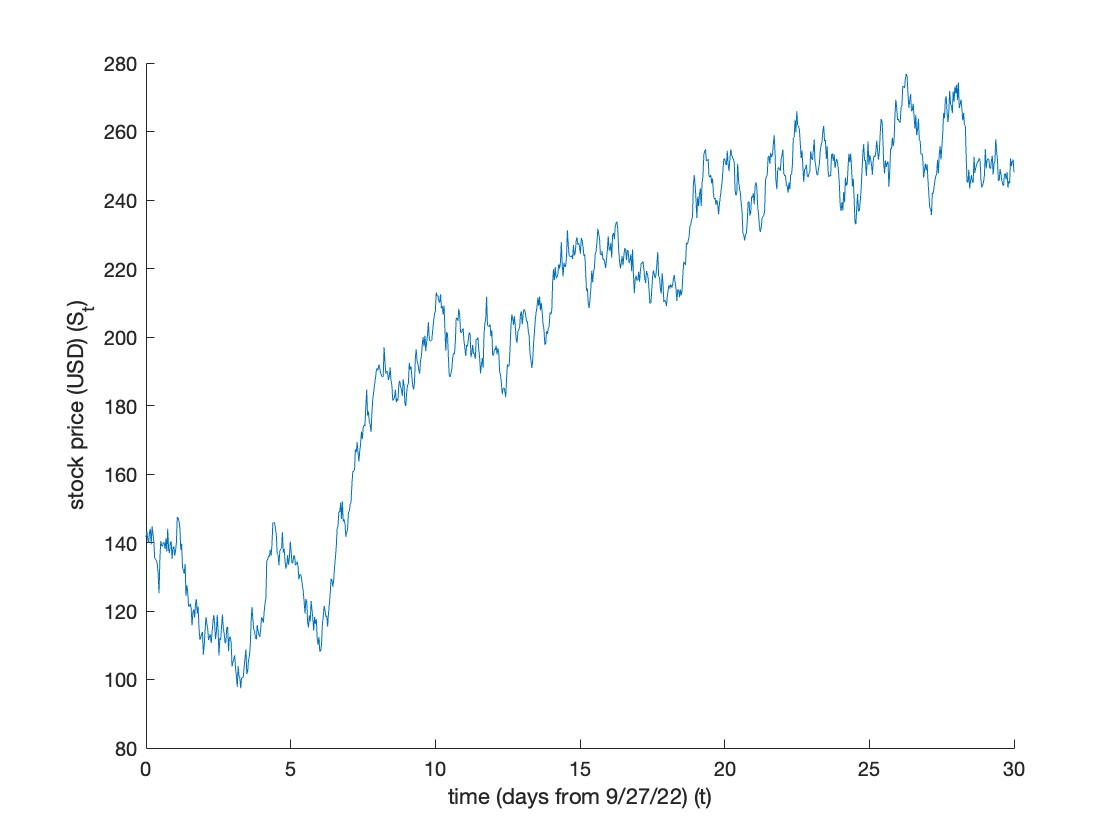
\includegraphics[width = 10cm]{Images/modelGraph.jpg}\]
	\begin{thebibliography}{1}
		\bibitem{Yahoo}
			Yahoo Finance,
			\textit{Alphabet Inc. (GOOG) Stock Price, News, Quote \& history - Yahoo Finance},
			New York, NY,
			2022.
		\bibitem{Stochastic}
			Gregory F. Lawler,
			\textit{Stochastic Calculus: An Introduction with Applications},
			Chicago, IL, 
			2014.
		\bibitem{Ito}
			Wenyu Zhang,
			\textit{Introduction to It\^o's Lemma},
			Ithaca, NY,
			May 6th, 2015
		\bibitem{Brownian}
			Andrea Chello,
			\textit{A Gentle Introduction to Geometric Brownian Motion in Finance},
			October 30th, 2020
		\bibitem{Random}
			Charles Zaiontz,
			\textit{Random Walk},
			2021
	\end{thebibliography}
\end{document}